% =====================================================================
%  Auditing the Lifecycle, Not the Transaction
%  Cost asymmetry, one-sided dispute resolution, and mocked-authentication
%  blind spots in a Soroban token-escrow contract family
%
%  COMPILATION STATUS: VERIFIED. Three pdflatex passes produce main.pdf at
%  nine pages with zero errors, zero undefined references, and zero undefined
%  citations. Binary: /Library/TeX/texbin/pdflatex (TeX Live, macOS arm64).
%
%  NUMBER PROVENANCE: every quantity in this manuscript appears in the
%  evidence tables of Section 6 or is derived from them by arithmetic that is
%  shown inline. Anything not so supported carries a literal TODO marker of
%  the form described in REFERENCES-NOTES.md. There are no other sources for
%  numbers in this document.
% =====================================================================
\documentclass[sigconf,review]{acmart}

\ccsdesc[300]{Software and its engineering~Software creation and management}
\ccsdesc[300]{Security and privacy~Formal security models}
\ccsdesc[200]{Social and professional topics~Computing / technology policy}

\keywords{smart contract audit, Soroban, Stellar, escrow, transaction cost,
authorization testing, dispute resolution, blockchain measurement}

% Declared explicitly so the manuscript is self-contained. acmart loads
% amsmath but not these three; \checkmark needs amssymb, \toprule needs
% booktabs, and the reproduction command blocks need listings with line
% breaking enabled for a two-column layout.
\usepackage{amssymb}
\usepackage{array}
\usepackage{booktabs}
\usepackage{listings}
\lstset{basicstyle=\ttfamily\small,breaklines=true,frame=none,
        xleftmargin=0pt,columns=fullflexible,showstringspaces=false}

% TODO(authorship): the audit was performed against the four repositories
% named in Section 4. No author names, affiliations, or contact addresses were
% provided with the audit materials, so the anonymous-submission form is used.
% Insert the real author block before submission; nothing is invented here.

\begin{document}

\title{Auditing the Lifecycle, Not the Transaction: Cost Asymmetry,
       One-Sided Dispute Resolution, and Mocked-Authentication Blind Spots
       in a Soroban Token-Escrow Contract Family}

% ----------------------------------------------------------------------------
% 1. ABSTRACT
% ----------------------------------------------------------------------------
\begin{abstract}
Token escrow on Soroban is usually evaluated one operation at a time: a
proposal names a handful of risky calls, and a test suite is read as evidence
that those calls are safe. We report the opposite result from an executed
audit of a Soroban token-escrow contract family. Reading the contract's own
recorded testnet fee data, the operation that moves the buyer's money into
escrow (\texttt{fund\_escrow}, 366{,}938 stroops) costs 20.6 times the
operation that moves it out (\texttt{release\_funds}, 17{,}791 stroops), while
the project's documentation asserts a near-constant per-transaction cost. The
same contract family contains a dispute mechanism that is entered
symmetrically by either party but resolved only in the buyer's favour: once an
escrow is \texttt{Disputed}, both the seller-side and buyer-side exits reject,
the only remaining transition returns 100\% of the amount to the buyer with no
fee, and no code path pays a disputed escrow's seller. Separately, every test
in the suite calls \texttt{env.mock\_all\_auths()}, under which
\texttt{require\_auth} succeeds for any caller; the test named
\texttt{test\_unauthorized\_refund} therefore passes on a later caller-identity
check and does not exercise authorization failure at all, so the suite's green
status overstates the authorization evidence it provides. We report these as
one methodological point: for Soroban escrow, the economically decisive and
security-critical behaviour sits in the transitions \emph{between} operations,
which per-operation threat models and per-operation tests both miss. All
monetary figures are on-chain stroop counts for a single observed lifecycle
($n=1$ per step). We assert no settlement latency, cost saving, mainnet
viability, or production readiness, because none is instrumented.
\end{abstract}

% ----------------------------------------------------------------------------
% 2. INTRODUCTION
% ----------------------------------------------------------------------------
\section{Introduction}
\label{sec:intro}

Escrow is the primitive that makes a tokenized cross-border payment
conditional: a buyer commits funds, a seller delivers, and a third party
refers the outcome to a rule. In a fiat corridor that rule is usually the
correspondent bank's. On a smart-contract platform the rule is the contract,
and the contract's lifecycle \emph{is} the trust model. This paper takes that
observation literally: we treat the lifecycle of an escrow contract as the
object of study, and we look at the cost and control flow \emph{between} the
operations that documentation and per-operation threat models normally
enumerate separately.

The subject is a Soroban (Stellar) token-escrow contract family, implemented in
Rust against \texttt{soroban-sdk} 26.1.1, with a second sibling repository
against 27.0.6. The family is a reasonable specimen rather than a convenient
one: it is a working, tested, testnet-deployed escrow with a fee mechanism, a
bounded error type, committed test snapshots, and a written dispute policy. Its
documentation makes explicit, checkable economic claims. That combination is
what allows the audit reported here to be unusually direct: the repository
records its own on-chain fee data, so the cost of each operation is a matter of
record rather than of modelling.

Three findings follow from reading that record together with the source.

\textbf{First, lifecycle cost is not uniform, and the documentation says it
is.} Across the seven recorded steps of one observed lifecycle, \texttt{fund\_
escrow} cost 366{,}938 stroops and \texttt{release\_funds} cost 17{,}791
stroops: a ratio of 20.6. The three escrow operations together account for
47.6\% of the 770{,}179 stroops that this one lifecycle cost, and a single
operation, \texttt{fund\_escrow}, accounts for 47.6\% of that lifecycle total
on its own. The project's own README asserts ``$\sim$\$0.00001 per
transaction'' and that gas is ``virtually \$0''. A flat per-transaction figure
cannot be approximately correct for a lifecycle whose recorded fees span a
factor of 40.1. We do not restate a dollar figure of our own, because the audit
materials contain no exchange rate with which to convert stroops; we make only
the structural claim, which requires no conversion.

\textbf{Second, the dispute mechanism is one-sided.} \texttt{raise\_dispute}
is callable by the buyer or the seller, so entry is symmetric. Resolution is
not: in state \texttt{Disputed}, \texttt{release\_funds} rejects and
\texttt{refund\_buyer} rejects, and the only accepted transition,
\texttt{auto\_refund\_if\_expired}, returns the full amount to the buyer with no
fee. The repository documents this as deliberate. It does not analyse the
economic consequence, which is that the contract contains no path in which a
disputed escrow pays its seller, and that a counterparty pricing this contract
rationally would decline to trade.

\textbf{Third, the test suite reports authorization coverage it does not
have.} Every test calls \texttt{env.mock\_all\_auths()}. Under mocked
authorization, \texttt{caller.require\_auth()} succeeds for any caller, so a
test that expects an authorization failure cannot fail for that reason. The
suite nonetheless contains a test named \texttt{test\_unauthorized\_refund}
that passes, and no test anywhere in the family asserts that
\texttt{release\_funds} rejects the seller.

These three findings are one finding. The operation that carries the
lifecycle's cost is not the operation the threat model interrogates; the
transition that decides who is paid is a terminal transition, not the dispute
entry that gets documented; and the property that would have caught both --- that
only the right principal may move funds --- is precisely the property the
standard Soroban test idiom disables. We state our contribution narrowly. We
have executed one test suite per repository, read one contract, and inspected
one set of on-chain fee records at $n=1$ per step. We claim a set of specific
defects and one methodological consequence, and we claim nothing about
settlement speed, cost savings against any payment rail, mainnet behaviour,
throughput, or production readiness, because the audit materials contain no
instrumentation for any of those quantities
(Section~\ref{sec:limitations}).

% TODO(related-work): a submission to a conference venue would situate these
% findings against the published literature on smart-contract escrow, Soroban
% fee structure, and the security of mock-based test oracles. No literature
% search was performed and no publication was available to the audit, so
% citing any specific work here would be fabrication. This paragraph is the
% honest marker of a missing related-work section. A companion artifact,
% REFERENCES-NOTES.md, records the same gap.

% ----------------------------------------------------------------------------
% 3. BACKGROUND
% ----------------------------------------------------------------------------
\section{Background: Soroban Escrow Mechanics}
\label{sec:background}

\subsection{Why the lifecycle, and not the transaction, is the unit of analysis}

In a fee model that is uniform per transaction, the cost of a payment protocol
is a function of how many transactions it needs, and the design question is
``how few?''. On Soroban the cost of a transaction is not uniform across
operations that a protocol author would consider interchangeable, because the
operations differ in what they must read, what they must write, and which
entries they must create. \texttt{fund\_escrow} moves value into the contract
and creates a trustline held by the contract; \texttt{release\_funds} moves
value out of a trustline that already exists. A designer who reasons per
operation sees four operations and prices them identically. A designer who
reasons per lifecycle sees that the lifecycle is dominated by its most
expensive step, and that the step which dominates it is the one that commits
the buyer's money.

The same argument applies to control flow. Escrow correctness is a property of
the transition relation, not of the guards on individual operations. An
operation can be individually correct and still be part of a lifecycle that
strands funds, because a guard that is correct in isolation may be the last
reachable transition.

\subsection{Operations, fee arithmetic, and the observable guards}

The contract family under study exposes four mutating operations. We describe
them only to the depth the source supports.

\texttt{create\_escrow} instantiates the record. \texttt{fund\_escrow}
transfers the escrowed amount from the buyer and places the contract in
\texttt{Funded}. \texttt{release\_funds} pays the seller and pays a protocol
fee to a treasury address. \texttt{refund\_buyer} returns the amount to the
buyer. A fifth entry point, \texttt{raise\_dispute}, moves an escrow into
\texttt{Disputed}, and \texttt{auto\_refund\_if\_expired} discharges an expired
one.

The fee is computed in integer arithmetic with truncation toward zero:
\begin{equation}
\label{eq:fee}
\mathrm{fee} \;=\; \left\lfloor \frac{\mathrm{amount} \times \mathrm{fee\_bps}}{10\,000} \right\rfloor ,
\qquad \mathrm{fee\_bps} \in [0,\, 1000].
\end{equation}
The upper bound \texttt{MAX\_FEE\_BPS = 1000} is a 10\% cap
(\texttt{lib.rs:11}); the rate used in the test suite is
\texttt{DEFAULT\_FEE\_BPS = 80}, a 0.8\% rate (\texttt{tests.rs:12}). The
formula appears at \texttt{lib.rs:199} and \texttt{lib.rs:226}. The remainder
of the amount goes to the seller. Equation~\ref{eq:fee} has no minimum-fee
term, which matters for small amounts (Finding~\ref{f:fee}).

Table~\ref{tab:guards} records the guard on each operation as observed in the
source. The last column is load-bearing: it states what the audit materials do
\emph{not} establish, so that the transition relation is not over-read.

\begin{table}[t]
\caption{Observed operation guards. The final column records what the audit
materials do not establish; the state type was not fully enumerated.}
\label{tab:guards}
\small
\begin{tabular}{@{}llll@{}}
\toprule
Operation & Location & Accepted input state & Not established \\
\midrule
\texttt{release\_funds}    & \texttt{lib.rs:186} & not \texttt{Disputed} & target state \\
\texttt{require\_auth}     & \texttt{lib.rs:231} & --- & enclosing function \\
caller-identity check     & \texttt{lib.rs:239} & --- & enclosing function \\
\texttt{refund\_buyer}     & \texttt{lib.rs:243} & not \texttt{Disputed} & target state \\
\texttt{raise\_dispute}    & \texttt{lib.rs:259} & not \texttt{Disputed} & prior states \\
\texttt{auto\_refund\_}\newline\textit{expired} &
  \texttt{lib.rs:311} & \texttt{Funded} or \newline \texttt{Disputed} &
  deadline value, \newline clock source \\
\bottomrule
\end{tabular}
\end{table}

% TODO(state-enum-enumeration): the state type was not fully enumerated in
% the audit materials. Only `Funded` and `Disputed` are named, and the states
% reached by release_funds and refund_buyer are unknown. Enumerate the full
% state type and its transitions from the source, and replace Table 1.

% TODO(auth-helper-callgraph): the audit materials give line numbers for the
% require_auth call (lib.rs:231) and the caller-identity check (lib.rs:239)
% but do not establish which function encloses them. The call graph of the
% authorization helper into refund_buyer and release_funds must be read from
% the source before the guard analysis in Table 1 can be completed.

% TODO(deadline-clock): auto_refund_if_expired admits Funded or Disputed, but
% the audit materials do not state the deadline field's source. Whether the
% deadline is a caller-supplied parameter or contract-stored is material to
% Finding F2 and must be read from the source.

\subsection{Testing idiom and the mocked authorization oracle}

The contract family is tested with the standard Soroban host test harness.
Every test begins by calling \texttt{env.mock\_all\_auths()}, which installs an
authorization mock: \texttt{require\_auth} and
\texttt{require\_auth\_for\_args} return success for any caller and any
argument, while recording the invocation. This is the correct default for tests
whose subject is business logic, because it lets a test set up state without
constructing signatures. It is the wrong oracle for a test whose subject is
authorization itself, because it removes the condition under test. A test
written against the mock can only ever fail for reasons other than the one it
names. Section~\ref{f:auth} returns to the consequences.

% ----------------------------------------------------------------------------
% 4. SYSTEM UNDER STUDY
% ----------------------------------------------------------------------------
\section{System under Study}
\label{sec:system}

\subsection{Contract shape}

The contract under study is a single-token escrow. Its error type
\texttt{EscrowError} has ten variants (\texttt{lib.rs:15--33}), among them a
fee-validation variant, \texttt{InvalidFee}, raised outside the accepted
$0 \le \mathrm{fee\_bps} \le 1000$ band. The contract is distributed as
\texttt{public/escrow.wasm}, 24{,}827 bytes, SHA-256
\texttt{a648e75a76dae8a8b04ab08fc60d2588c68a2ffb1e043cdd106ce910a777d2c1}.
The build artifact that produced that hash is not committed to the repository,
so the deployed bytecode's byte-identity cannot be checked from the repository
alone; the hash is recorded here as the audit's own observation.

The test suite comprises 26 committed \texttt{test\_snapshots} JSON files under
\path{contracts/contracts/escrow/test_snapshots/tests/}, generated by
\texttt{soroban-sdk} 26.1.1.

% TODO(wasm-provenance): the 24,827-byte artifact and its SHA-256 are recorded
% from the audit environment. Because contracts/target/.../escrow.wasm is not
% committed, no reader can confirm that the committed source, the recorded
% hash, and any deployed contract are the same object. Commit the build
% artifact, or publish a reproducible build with a pinned toolchain and
% lockfile, so byte-identity becomes checkable.

\subsection{Deployment evidence and version drift}

Three testnet proof documents record three different contract addresses for
this family, which is the clearest single indication that the deployed artifact
changed across the audit period.

\begin{table}[t]
\caption{Testnet escrow proofs. Three documents, three contract addresses. The
per-transaction fee data used in Section~\ref{sec:measurements} was recorded
against the first of these, which is not the address the README calls current.}
\label{tab:proofs}
\small
\begin{tabular}{@{}llrl@{}}
\toprule
Proof document & Asset & Amount & Contract \\
\midrule
\texttt{E2E-PROOF.md} &
  \texttt{BREAD}, self-issued, 7 dp &
  20 \texttt{BREAD} \newline $(200{,}000{,}000)$ &
  \texttt{CB7I2GUR}\dots \\
\texttt{E2E-USDC-PROOF.md} &
  Circle \texttt{USDC} &
  5 \texttt{USDC} \newline $(50{,}000{,}000)$ &
  \texttt{CBY6UC4I}\dots \\
\texttt{E2E-FEE-PROOF.md} &
  Circle \texttt{USDC} &
  0.05 \texttt{USDC} \newline $(500{,}000)$ &
  \texttt{CAFG7VWE}\dots \\
\bottomrule
\end{tabular}
\end{table}

The README identifies the third address, \texttt{CAFG7VWENECKXXS\allowbreak RH64G536IG4CD3\allowbreak ALJO3U6HUAN4P5\allowbreak JPMC4EXOUPHKO},
as the current contract, at version~9. The fee figures in
Table~\ref{tab:fees} were recorded against
\texttt{CB7I2GURQDV4Q7\allowbreak YAT2PZAG3ZNFQJ\allowbreak 37GI6MWZ4P3W7\allowbreak SUCJZPSHP2G6L6J}. This
matters for Finding~\ref{f:cost}: the ratio reported below is a property of one
observed lifecycle on an earlier address of the same family, and has not been
re-measured against the address the project ships as current. Only the first
proof carries a date, 2026-09-25; the other two carry none in the audit
materials.

The \texttt{E2E-FEE-PROOF.md} document reports a conservation check on the
0.05 \texttt{USDC} escrow: $0.0124 + 5.0496 + 0.0004 + 0 = 5.0624$. The
arithmetic is correct. The per-term semantics are not established, so the paper
does not interpret which term, if any, is a protocol fee, or at what rate.

% TODO(fee-proof-decomposition): E2E-FEE-PROOF.md reports four terms summing to
% 5.0624 against a 0.05 USDC escrow. The label and provenance of each term are
% not in the audit materials. Until each term is identified, it cannot be
% checked against MAX_FEE_BPS = 1000, and the conservation check cannot confirm
% that the cap is respected on the only real-asset fee proof in the family.
% Sample size is one.

% TODO(usdc-decimals): the 7-decimal place value is established for BREAD
% only. The decimal precision of the Circle USDC asset as used in
% E2E-USDC-PROOF.md and E2E-FEE-PROOF.md is not stated in the audit materials
% and is required to interpret the base-unit amounts in Table 3 as whole units.

% TODO(contract-version-alignment): re-run the seven-step fee measurement
% against CAFG7VWEN... (the version the README ships as current) and report
% both sets of figures. Until then, Finding F1's ratio is version-scoped to
% CB7I2GUR... and must not be generalised across the family's versions.

% ----------------------------------------------------------------------------
% 5. METHOD
% ----------------------------------------------------------------------------
\section{Method}
\label{sec:method}

\subsection{Reproduction procedure}

The audit re-ran each repository's own suite and read the artifacts the
repositories commit. No test was written to make a finding pass, and no failing
test was modified. Commands and toolchain versions are given in
Section~\ref{sec:repro} and in the repository \texttt{README.md}.

\subsection{Analytic derivations}

Four derivations are used in this paper, and each is a plain arithmetic
identity over quantities already in the audit materials, shown inline at the
point of use:
\begin{enumerate}
\item the ratio of two recorded fees, $\mathrm{fee}(\texttt{fund\_escrow}) /
      \mathrm{fee}(\texttt{release\_funds})$;
\item the total of the seven recorded fees, and the share of that total
      contributed by one escrow operation;
\item the ratio of the largest to the smallest recorded fee across the
      lifecycle;
\item the largest amount for which Equation~\ref{eq:fee} truncates to zero at
      the default rate, which is $\lfloor (10\,000-1) / 80 \rfloor = 124$ base
      units.
\end{enumerate}

The figure in this paper is generated by a script that reads the recorded fee
table as a committed CSV and re-checks each of these derivations against the
artifact values before emitting the figure; the script aborts if any
derivation disagrees (Section~\ref{sec:repro}).

% TODO(fee-resource-breakdown): the audit materials record only the aggregate
% fee charged per transaction. They do not decompose it into the resource
% classes that drive it. The paper therefore states WHERE the 20.6x ratio
% comes from (a transfer that creates a trustline held by the contract plus an
% escrow-state write) and not WHY in resource terms. Producing the
% per-resource fee breakdown, from transaction simulation or resource
% metering, is required before any mechanism claim can be made.

% ----------------------------------------------------------------------------
% 6. MEASUREMENTS
% ----------------------------------------------------------------------------
\section{Measurements}
\label{sec:measurements}

\subsection{On-chain fees, $n=1$ per step}

Table~\ref{tab:fees} reproduces the only per-transaction fee data that exists
for this family: the seven recorded steps of a single escrow lifecycle on
Stellar testnet, transcribed from \texttt{E2E-PROOF.md:70--95}. Each row is one
observed transaction. There is no replication, so these are descriptions of one
lifecycle, not samples from a distribution; no confidence interval, variance,
or percentile is computable from them and none is reported.

\begin{table}[t]
\caption{Recorded testnet fees for one observed escrow lifecycle,
$n=1$ per step. Source: \texttt{E2E-PROOF.md:70--95}, contract
\texttt{CB7I2GUR}\dots. Ledger numbers are sequence numbers, not timestamps.}
\label{tab:fees}
\small
\begin{tabular}{@{}lrl@{}}
\toprule
Step & Fee (stroops) & Ledger \\
\midrule
S1 \texttt{deploy\_asset\_and\_sac}   & 183{,}215 & 4{,}869{,}181 \\
S2 \texttt{buyer\_trust\_sac}        &  14{,}202 & 4{,}869{,}189 \\
S3 \texttt{seller\_trust\_sac}       &  14{,}202 & 4{,}869{,}192 \\
S4 \texttt{mint}                     &   9{,}140 & 4{,}869{,}199 \\
\midrule
S5 \texttt{create\_escrow}           & 164{,}691 & 4{,}869{,}212 \\
S6 \texttt{fund\_escrow}             & \textbf{366{,}938} & 4{,}869{,}217 \\
S7 \texttt{release\_funds}           & \textbf{17{,}791} & 4{,}869{,}223 \\
\bottomrule
\end{tabular}
\end{table}

\begin{figure}[t]
\centering
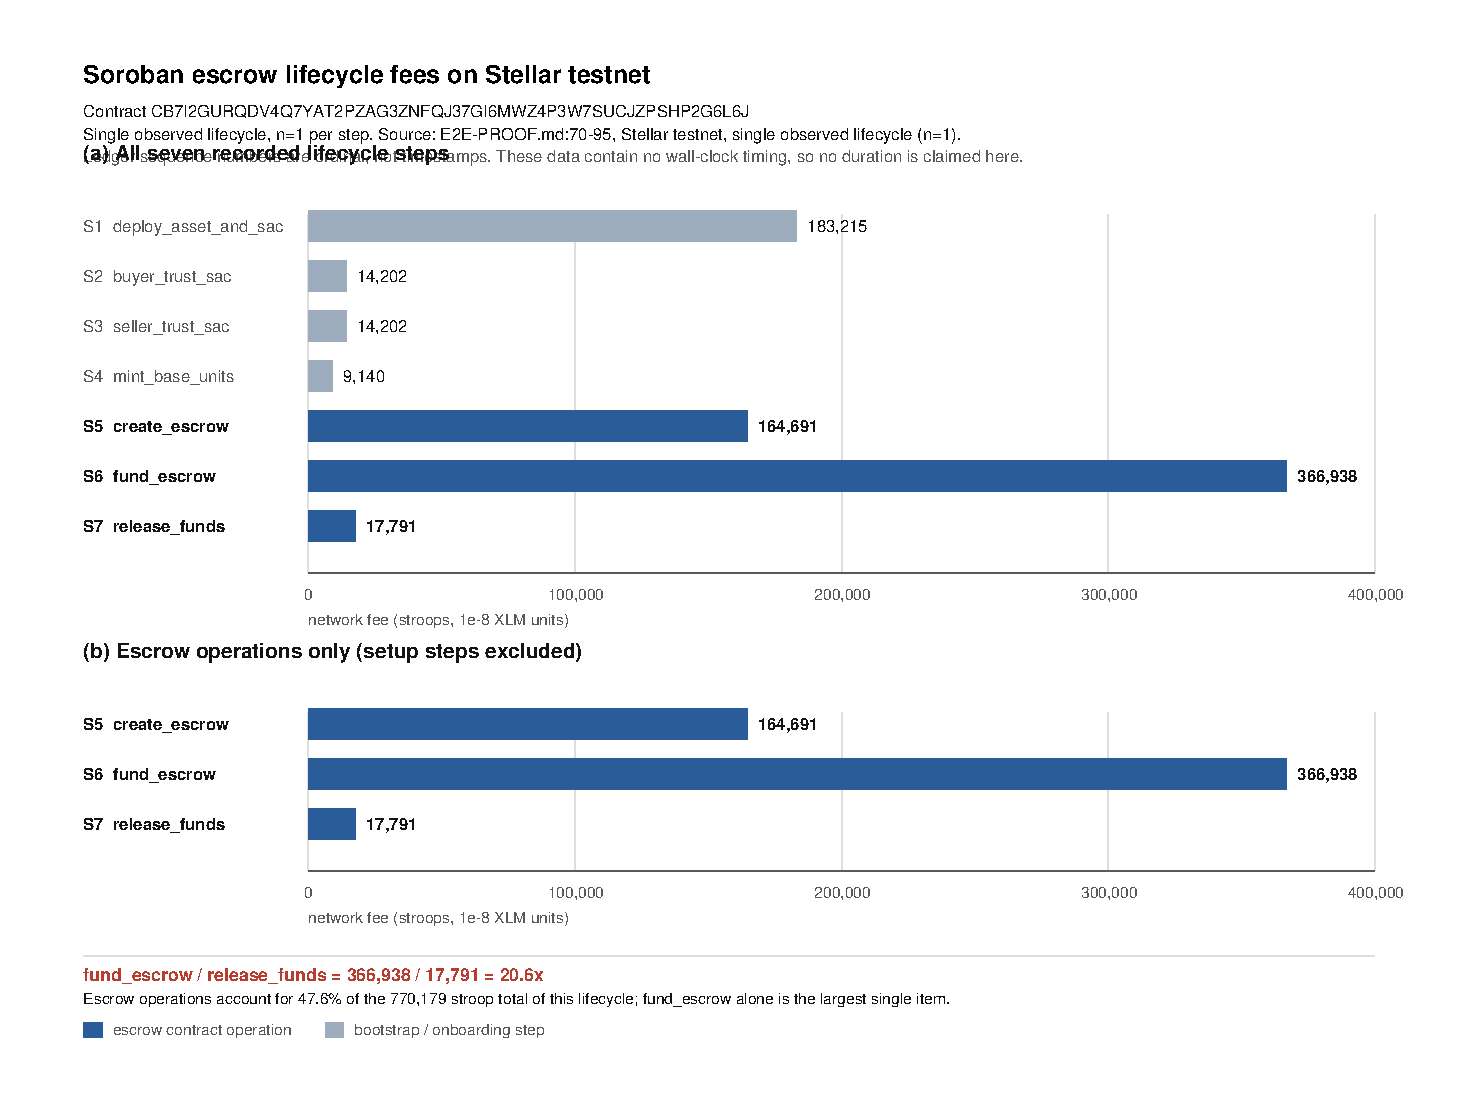
\includegraphics[width=\columnwidth]{figures/lifecycle_fees.pdf}
\caption{Recorded network fees for the seven steps of one observed escrow
lifecycle on Stellar testnet, $n=1$ per step. Panel (b) isolates the three
escrow operations. Derived from \texttt{E2E-PROOF.md:70--95}; generated by
\texttt{figures/make\_figures.py} from \texttt{figures/data/lifecycle\_fees.csv}.
Because $n=1$, no statement about fee variation is made or supported.}
\label{fig:fees}
\end{figure}

Figure~\ref{fig:fees} plots the same data. Three observations follow directly,
and each is arithmetic over Table~\ref{tab:fees}:
\begin{align}
\frac{\mathrm{fee}(\texttt{fund\_escrow})}{\mathrm{fee}(\texttt{release\_funds})}
  &= \frac{366{,}938}{17{,}791} = 20.62 \approx 20.6\times, \label{eq:ratio} \\
\sum_{i=1}^{7} \mathrm{fee}(S_i) &= 770{,}179 \ \text{stroops}, \label{eq:sum} \\
\frac{\mathrm{fee}(\texttt{fund\_escrow})}{\sum_{i=1}^{7}\mathrm{fee}(S_i)}
  &= 0.4764 \approx 47.6\%, \label{eq:share} \\
\frac{\max_i \mathrm{fee}(S_i)}{\min_i \mathrm{fee}(S_i)}
  &= \frac{366{,}938}{9{,}140} = 40.15 \approx 40.1\times. \label{eq:span}
\end{align}

The absolute difference between the two escrow transfers is
$366{,}938 - 17{,}791 = 349{,}147$ stroops. The two operations also differ
from each other in direction, and the paper makes no claim about whether the
asymmetry would persist at other amounts, other assets, or other
addresses.

The ledger column in Table~\ref{tab:fees} is an \emph{ordinal} sequence number.
The seven steps span 42 ledger numbers, and the audit materials contain no
wall-clock timing of any kind. Ledger sequence numbers cannot be converted to
durations from the available data, and this paper reports no duration.

\subsection{Executed tests}

Table~\ref{tab:tests} lists every test command executed during the audit. A
failing command is reported as a failing command.

\begin{table*}[t]
\caption{Executed test commands. \checkmark\ marks a passing run; failures are
reported with their counts. Totals refer only to passing runs.}
\label{tab:tests}
\small
\begin{tabular}{@{}llllrl@{}}
\toprule
Repository & Command & Outcome & SDK & Runtime & Note \\
\midrule
\texttt{breadline-protocol} & \texttt{cargo test} &
  \checkmark\ 26 passed, 0 failed & 26.1.1 & 0.91\,s & escrow contract suite \\
\texttt{proofdrop} & \texttt{npm test} &
  \checkmark\ 38 passed, 0 failed & --- & --- &
  shared 8/8, api 30/30 \\
\texttt{pactopay} & \texttt{cargo test} &
  \checkmark\ 8 passed, 0 failed & 27.0.6 & 0.63\,s & contract suite only \\
\texttt{pactopay} & \texttt{npx vitest run} &
  \textbf{failed} 9 of 11 files, 5 of 20 tests & --- & --- & integration \\
\texttt{pactopay} & \texttt{npx playwright test} &
  \textbf{failed} 8 failed, 4 skipped, 14 passed & --- & --- & end-to-end \\
\texttt{niko-sun-stellar} & not executed & --- & --- & --- &
  toolchain time ceiling \\
\bottomrule
\end{tabular}
\end{table*}

Seventy-two tests passed in total: 26, 38, and 8. The \texttt{proofdrop} suite
is 100\% mocked, runs at $n=1$, and uses an in-memory store. The
\texttt{pactopay} result is the informative one: its Rust suite is green while
its TypeScript integration and end-to-end suites fail, which is consistent with
the two liveness defects that the Rust suite does not cover
(Section~\ref{f:cost} and Section~\ref{sec:limitations}). No green continuous
integration run exists for any of the four repositories.

% TODO(ci-baseline): no repository in the family has a green CI run of record.
% The suites were executed locally. Until CI is green, "the test suite passes"
% is a statement about one machine at one moment. Record a CI run per
% repository and cite the run URLs.

\subsection{Test snapshots and the testnet records}

Twenty-six \texttt{test\_snapshots} JSON files are committed. Three testnet
proof documents record escrow executions against three contract addresses
(Table~\ref{tab:proofs}). These are the artifacts that exist; the audit
records no mainnet execution of any kind.

% ----------------------------------------------------------------------------
% 7. FINDINGS
% ----------------------------------------------------------------------------
\section{Findings}
\label{sec:findings}

\subsection{F1: Lifecycle cost asymmetry invalidates the flat per-transaction
cost claim}
\label{f:cost}

\textbf{Evidence.} \texttt{fund\_escrow} cost 366{,}938 stroops and
\texttt{release\_funds} cost 17{,}791 stroops in the same lifecycle
(Table~\ref{tab:fees}), a ratio of 20.6 by Equation~\ref{eq:ratio}. The
largest-to-smallest spread across the seven recorded fees is 40.1
(Equation~\ref{eq:span}). The three escrow operations account for 47.6\% of
the lifecycle's 770{,}179 stroops (Equations~\ref{eq:sum} and
\ref{eq:share}), and \texttt{fund\_escrow} alone is 47.6\% of that total.

\textbf{Consequence.} The project's documentation asserts ``$\sim$\$0.00001 per
transaction'' and that gas is ``virtually \$0''. We reproduce those figures
here only as claims the audit falsifies, and the falsification is structural:
a single per-transaction constant cannot be approximately correct for a
lifecycle whose own recorded fees span a factor of 40.1. The economic content
of this finding is not that fees are high --- on testnet, with the amounts in
Table~\ref{tab:fees}, the absolute magnitudes are small --- but that a
cost-uniformity assumption is false, and that it is the assumption a cost model
built on it would rest on. We do not restate a dollar figure of our own,
because converting stroops to a fiat amount requires an exchange rate that the
audit materials do not contain.

The design consequence is specific. The step that commits the buyer's money is
the expensive step: 2.2 times \texttt{create\_escrow} and 20.6 times
\texttt{release\_funds}. A protocol that splits a payment into many small
escrows pays this cost once per escrow, while a protocol that batches pays it
once. A cost model that prices all four operations identically predicts none of
this.

Two scope limits are load-bearing. First, the measurement is $n=1$ per step on
one address of the family, not the address the README ships as current
(Table~\ref{tab:proofs}); the ratio is therefore version-scoped.
Second, the recorded fee is an aggregate. The audit materials do not
decompose it into resource classes, so this finding identifies which operation
is expensive and does not claim why.

% TODO(fee-replication): n=1 per step. Repeat each of the seven steps at
% least 30 times per (amount, asset, address) and report the distribution,
% median, and p95. Until then no statement about typical fee or fee stability
% is supportable, and none is made.

% TODO(mainnet-fees): all records are testnet. Testnet fee schedules and
% resource pricing are not evidence of mainnet fee behaviour, and the family
% has no mainnet deployment. Measuring the same seven steps on mainnet is
% required before any statement about production cost.

\subsection{F2: One-sided dispute resolution is a dispute-extraction
surface}
\label{f:dispute}

\textbf{Evidence.} \texttt{raise\_dispute} (\texttt{lib.rs:259}) is callable by
the buyer or the seller and sets state \texttt{Disputed}. In
\texttt{Disputed}, \texttt{release\_funds} (\texttt{lib.rs:186}) and
\texttt{refund\_buyer} (\texttt{lib.rs:243}) both reject.
\texttt{auto\_refund\_\allowbreak if\_\allowbreak expired} (\texttt{lib.rs:311}) accepts
\texttt{Funded} or \texttt{Disputed} and returns the amount to the buyer, and
the test suite records that the returned amount carries no fee. The repository
documents the behaviour as deliberate at \texttt{lib.rs:296--303}.
Concatenating the three guards, there is no reachable state in which a
disputed escrow pays its seller.

\textbf{Consequence.} Entry to the dispute path is symmetric; resolution is
not. A buyer who raises a dispute and lets the deadline pass recovers 100\% of
the amount at no fee. This is not a rounding loss or a fee-maximising
edge case: it is the full amount, and the seller's only recourse is a path
that does not exist. Two consequences follow for protocol design. First, an
escrow built on this contract is a credit instrument against the seller for
the buyer's dispute decision, so a seller must price that decision out of the
consideration, or not trade. Second, the README describes the mechanism more
generously (\texttt{README.md:286}) than the code behaves, which is the
defect a reader relying on the documentation would inherit. The repository
documents the behaviour; it does not analyse the consequence. That gap, not
the behaviour alone, is the finding.

We state this as a property of the transition relation. We did not execute an
attack against it, and no evidence in the audit materials shows anyone
exploiting it.

% TODO(dispute-exit): the honest counter-argument to F2 is that a symmetric
% dispute path may have been out of scope for the deliverable. Test that
% reading by asking the project maintainers whether a seller-side resolution
% path was planned and deferred. If it was deferred, F2 becomes a scoping
% defect rather than a design defect, and the paper should say so.

\subsection{F3: Truncating fee arithmetic creates a zero-fee region at small
amounts}
\label{f:fee}

\textbf{Evidence.} The fee is
$\lfloor \mathrm{amount} \times \mathrm{fee\_bps} / 10{,}000 \rfloor$
(\texttt{lib.rs:199}, \texttt{lib.rs:226}) with no minimum-fee term. The suite
asserts that releasing 1{,}000 base units at 80\,bps sends 8 to the treasury
and 992 to the seller (\texttt{tests.rs:193--196}, \texttt{tests.rs:849--852}),
and that releasing 3{,}000 base units charges 24 (\texttt{tests.rs:794}). The
suite also asserts the boundary case: an amount of 1 base unit at 80\,bps
produces a fee of 0 and pays the seller the full 1 base unit
(\texttt{tests.rs:1082--1113}). The cap boundary is enforced on the rate and
not on the fee: 1{,}000\,bps is accepted and 1{,}001\,bps raises
\texttt{InvalidFee} (\texttt{tests.rs:921--963}).

\textbf{Consequence.} Equation~\ref{eq:fee} truncates to zero whenever
$\mathrm{amount} \times \mathrm{fee\_bps} < 10{,}000$. At the default rate of
80\,bps the largest such amount is $\lfloor (10{,}000-1)/80 \rfloor = 124$ base
units; at 1{,}000\,bps it is 9. \emph{This threshold is derived from the
formula and the default rate, not itself an executed test result}: the suite
exercises only the single-amount case at 1 base unit. The cap is a ceiling on
the rate, and the contract has no floor on the fee, so a caller can construct
an arbitrarily small escrow that moves value with no protocol fee.
Downstream, any arithmetic that assumes a fee was charged for a release --- a
treasury reconciliation that sums observed fees, or a screening rule keyed on
fee presence --- has an unmodelled case at amounts at or below the threshold.
For the \texttt{BREAD} deployment, which the audit materials establish to have
7 decimal places, 124 base units is below the smallest representable trade in
any realistic unit; the point is the shape of the mechanism, not this
particular bound.

\subsection{F4: Mocked authorization masks the authorization coverage the
suite appears to report}
\label{f:auth}

\textbf{Evidence.} Every test in the suite calls
\texttt{env.mock\_all\_auths()}. Under the mock, \texttt{caller.require\_auth}
(\texttt{lib.rs:231}) returns success for any caller. The suite contains
\texttt{test\_unauthorized\_refund} (\texttt{tests.rs:348}), and that test
passes --- but it passes because of a caller-identity check at
\texttt{lib.rs:239}, not because an authorization was required and refused. No
test in the family asserts that \texttt{release\_funds} rejects the seller, and
no test anywhere in the family exercises a \texttt{require\_auth} failure.

\textbf{Consequence.} The suite is green, and its green status is not evidence
about authorization. The two mechanisms are different:
\texttt{require\_auth} is a signature-authorization gate whose rejection path
the mock deletes, while the check at \texttt{lib.rs:239} is a
caller-identity comparison against a stored party. \texttt{test\_unauthorized\_refund}
therefore does provide a real result --- only the recorded buyer can
\texttt{refund\_buyer} --- but it provides that result through a mechanism it does
not name,
and it provides no evidence at all about the signature-authorization gate.

This is the finding with the widest reach, because it is about the test
infrastructure rather than about this contract. \texttt{mock\_all\_auths} is
the correct default for testing business logic, and it is what almost every
Soroban test suite uses. A suite can be large, thorough-looking, and entirely
green while providing zero evidence about authorization enforcement, and a
reviewer reading test counts and names has no signal that distinguishes the two
cases. A test whose name asserts a property the harness has disabled is worse
than no test, because it is counted as coverage.

% TODO(negative-auth-test): write the tests the suite lacks, using
% soroban-sdk's auth primitives without the mock (for example by constructing
% the test so that require_auth is reached with a non-matching key, or by
% using mock_auths with an explicit failing entry). Required cases: (a)
% release_funds rejects a caller that is not the recorded seller; (b)
% release_funds rejects a caller that is the seller but supplies no valid
% authorization; (c) refund_buyer likewise; (d) raise_dispute and
% auto_refund_if_expired likewise. Without these, F4 stands as an observation
% about the suite and not as a fixed defect.

% TODO(negative-auth-test-scan): the audit established that every test calls
% mock_all_auths by reading the suite. Re-verify mechanically (a test that
% constructs its own SorobanAuth would be an exception) and record the search
% command in the artifact so the claim is independently checkable.

% TODO(dust-threshold-test): confirm the derived threshold of 124 base units
% at 80 bps with a parametrized sweep over amounts 0..200, asserting the fee
% at each. The paper currently derives this from the formula; the executed
% evidence is the single-amount case at tests.rs:1082-1113.

% ----------------------------------------------------------------------------
% 8. THREAT MODEL
% ----------------------------------------------------------------------------
\section{Threat Model Discussion}
\label{sec:threat}

This section is analysis, not a report of exploited attacks. The audit
performed no penetration test, defined no adversary, and ran no adversarial
scenario against the deployed contracts. No evidence in the audit materials
indicates that any party exploited any vector below. Each item states what the
findings in Section~\ref{sec:findings} make \emph{reachable or visible} as a
property of the code, and stops there.

\textbf{T1 --- Dispute extraction (from F2).} The transition relation admits a
path from \texttt{Funded} to full buyer recovery with no seller payment, taken
by raising a dispute and expiring. The cost to the actor is one transaction
and the passage of the deadline. The consequence for a protocol built on this
contract is a value transfer that the protocol cannot prevent, which is a
pricing problem for the seller and a control problem for the integrator.

\textbf{T2 --- Liveness loss in the sibling contract
(\texttt{pactopay}).} The audit found two liveness defects in the sibling
contract: it has no deadline field, so funds can lock indefinitely; and a
\texttt{Disputed} milestone has no outgoing transition, so funds are
unrecoverable in both directions. Neither is covered by a test. These are
availability properties, and they are the class of defect the mock-based suite
is least likely to surface, because a test that never asserts a deadline or an
outgoing transition cannot fail for either.

% TODO(pactopay-liveness-tests): neither pactopay liveness defect is covered
% by a test. Add (a) a test asserting that an expired escrow with no deadline
% field is recoverable, which requires first adding the field, and (b) a test
% asserting that every milestone has a reachable outgoing transition, which
% fails today on the Disputed milestone. The Rust suite is green while both
% defects are present, which is the point: the suite does not ask.

\textbf{T3 --- Fee-free micro-escrow (from F3).} The absence of a minimum fee
means the protocol's own fee mechanism has a blind region at small amounts, and
the number of distinct escrow records a caller can create and release is not
bounded by any fee the protocol collects. The paper makes no claim about
whether this is reachable at a volume that matters; no volume measurement
exists.

\textbf{T4 --- Assurance inflation (from F4).} This is a vector against the
\emph{evidence}, not against the contract. A green suite with named tests that
do not exercise the property they name is consumed as authorization evidence by
reviewers, integrators, and funders who have no way to detect the gap from the
test output. The cost of the gap is paid downstream, in an integration that was
reviewed against evidence that did not exist.

F1 does not appear in this list as an attack, and should not be read as one. It
is a cost-structure property. Its relevance to security is indirect and worth
stating precisely: a threat model that budgets effort per operation, guided by a
flat per-transaction cost, will spend its attention on the operations the
documentation discusses. Finding~\ref{f:cost} shows that the operation which
commits the buyer's money is the expensive one, and Finding~\ref{f:dispute}
shows that the operation which decides who is paid is a terminal transition.
Both are missed by a per-operation view.

% TODO(threat-model): the audit defines no adversary. A threat model requires
% at least: actor classes (buyer, seller, integrator, funder, malicious
% deployer), their capabilities (what they can call and with whose
% authorization), and their incentives. None was provided with the audit
% materials. The vectors above are therefore code properties, not modelled
% attacks, and this section must not be described as a threat model in a
% submission until an adversary model exists.

% ----------------------------------------------------------------------------
% 9. LIMITATIONS
% ----------------------------------------------------------------------------
\section{Limitations}
\label{sec:limitations}

This section is load-bearing. The findings in Section~\ref{sec:findings} are
defects with consequences; the statements below are absences, and an absence
cannot be repaired by argument. A reader deciding whether to rely on this work
should read this section before the findings.

\subsection{No latency instrumentation exists anywhere}
The repository contains no latency instrumentation. A search for
\texttt{Date.now}, \texttt{performance.now}, \texttt{elapsed},
\texttt{median}, and \texttt{p95} returns four hits, all in unrelated UI logic.
There is no \texttt{performance.now()}, no \texttt{elapsed}, no
\texttt{median}, and no \texttt{p95} in the codebase. The README's
``$<3.5$\,s median testnet settlement'' has no measuring code behind it, and
this paper reports no settlement latency, settlement speed, or completion time
of any kind. The ledger numbers in Table~\ref{tab:fees} are ordinal sequence
numbers and are not convertible to durations from the available data.

\subsection{Sample size}
Every measurement in Section~\ref{sec:measurements} is $n=1$ per step. There
are no distributions, no repeated trials, and no confidence intervals. The
value 20.6 in Equation~\ref{eq:ratio} is the ratio of two single observations.
It is not an estimate of a population ratio, and its reproducibility across
runs, amounts, assets, and contract versions is unknown.

\subsection{Network}
All three escrow proofs are testnet. Nothing in this paper establishes mainnet
behaviour, real fee markets, or real liquidity in the assets involved. The
\texttt{BREAD} asset in the fee measurement is self-issued by the project, and
the \texttt{USDC} proofs reference Circle-issued \texttt{USDC} as represented on
a test network, which establishes nothing about the mainnet asset.

\subsection{Verification}
There is no threat-model adversary, no penetration test, and no formal
verification of the contract. Section~\ref{sec:threat} is analysis. No executed
attack is reported anywhere in this paper.

\subsection{Untested deployment path}
The per-user deployment path --- the mechanism the application actually uses ---
was never executed. \texttt{README.md:97} states that it requires a wallet
signature. The fee data in Table~\ref{tab:fees} comes from a different,
operator-side path.

\subsection{Test-suite scope}
The \texttt{proofdrop} suite is 100\% mocked, runs at $n=1$, and uses an
in-memory store. The \texttt{pactopay} TypeScript integration and end-to-end
suites fail (Table~\ref{tab:tests}). No repository in the family has a green
continuous integration run of record. The two \texttt{pactopay} liveness
defects are not covered by any test.

\subsection{Artifact and version identity}
The compiled \texttt{escrow.wasm} is not committed, so byte-identity of the
deployed artifact cannot be checked from the repository. The fee measurement was
taken against \texttt{CB7I2GUR}\dots, while the address the README ships as
current is \texttt{CAFG7VWEN}\dots. Findings are scoped accordingly.

\subsection{Unsupported claims left in the repository}
The repository states that the economics are ``85\% cheaper'' than SWIFT with a
flat \$45 charge and a 5.9\% spread. These are unsourced hardcoded constants in
the source. No comparison against any published price for any payment rail ---
SWIFT, PayPal, SPEI, PIX --- exists in the audit materials. This paper does not
repeat those figures as results. The word ``cheap'' is not used of this system
anywhere in this paper, because no comparison was performed.

% TODO(latency-instrumentation): instrument a settlement path with
% performance.now() or an equivalent monotonic clock, and record per-stage
% timings. Until then no latency claim of any kind is admissible, including in
% the README. Suggested: emit a JSON receipt per lifecycle with
% create/fund/release wall-clock deltas, then aggregate with median and p95
% over at least 30 lifecycles.

% TODO(economics-baseline): the economics comparison is unsourced. Any claim
% of cost saving requires a cited, dated price for the comparator rail and a
% stated currency conversion rate, with the rate and date recorded alongside
% the measurement. This paper deliberately asserts no saving.

% TODO(stroop-fiat): converting stroops to a fiat amount requires an XLM price
% and a date. Neither is in the audit materials, so this paper states fees in
% stroops only. Any monetary restatement must record the rate, its source, and
% its date.

% TODO(per-user-deploy): execute the per-user deployment path that
% README.md:97 describes, capture its transaction hashes, and measure its fee
% separately. The per-user path may have a different cost structure from the
% operator-side path measured in Table 3, which would change the scope of F1.

% TODO(related-work): see the marker in Section 1. A related-work section
% requires a real literature search; none was performed.

% TODO(registry-provenance): the reference list in Section 12 names software
% artifacts by repository name, contract address, and version. Retrieval
% metadata for the SDK crates (registry URL, release date) and for the
% repositories themselves was not available and is not asserted. Add it before
% submission so the references are resolvable.

% ----------------------------------------------------------------------------
% 10. REPRODUCTION
% ----------------------------------------------------------------------------
\section{Reproduction}
\label{sec:repro}

\subsection{Commands}

\begin{lstlisting}[language=bash]
# Contract suites
cd breadline-protocol && cargo test      # 26 passed, 0 failed; sdk 26.1.1
cd proofdrop        && npm  test         # 38 passed, 0 failed
cd pactopay         && cargo test        # 8 passed, 0 failed;  sdk 27.0.6

# Sibling suites, reported as failures
cd pactopay && npx vitest run            # failed: 9/11 files, 5/20 tests
cd pactopay && npx playwright test       # failed: 8 failed, 4 skipped, 14 passed

# Claimed-but-uninstrumented: returns four hits, all unrelated UI logic
grep -rniE "Date\.now|performance\.now|elapsed|median|p95" .

# Fee table, decoded from the repository's own proof document
sed -n '70,95p' E2E-PROOF.md
\end{lstlisting}

\subsection{Figure and derivation check}

The figure is generated from a committed CSV, and the script re-checks every
derived quantity in Section~\ref{sec:measurements} against the artifact values
before writing output. It exits non-zero if any check fails.

\begin{lstlisting}[language=bash]
cd figures
python3 make_figures.py --verify   # print derivations, write nothing
python3 make_figures.py            # write lifecycle_fees.pdf
\end{lstlisting}

\subsection{Artifacts}

Table~\ref{tab:artifacts} lists what the audit read and what could not be
checked.

\begin{table}[t]
\caption{Artifact provenance. Hashes are recorded where the audit established
them; ``not committed'' means byte-identity is not checkable from the
repository.}
\label{tab:artifacts}
\small
\begin{tabular}{@{}>{\raggedright\arraybackslash}p{0.30\linewidth}%
                 >{\raggedright\arraybackslash}p{0.66\linewidth}@{}}
\toprule
Artifact & Provenance \\
\midrule
\texttt{lib.rs}, \texttt{tests.rs} & source, cited by line \\
\texttt{E2E-PROOF.md} & fee table, lines 70--95 \\
\texttt{E2E-USDC-PROOF.md}, \newline \texttt{E2E-FEE-PROOF.md} & escrow proofs \\
\texttt{test\_snapshots}/ & 26 committed JSON files \\
\texttt{public/escrow.wasm} & 24{,}827 bytes; SHA-256 \newline
  \texttt{a648e75a76dae8a8} \newline
  \texttt{b04ab08fc60d2588c} \newline
  \texttt{68a2ffb1e043cdd1} \newline
  \texttt{06ce910a777d2c1}; \newline
  build artifact \emph{not committed} \\
\texttt{figures/data/}\newline \texttt{lifecycle\_fees.csv} & fee table, verbatim \\
\texttt{figures/make\_figures.py} & figure + derivation checks \\
\bottomrule
\end{tabular}
\end{table}

\subsection{Build status}
This manuscript has been compiled. Three \texttt{pdflatex} passes on
macOS arm64 with TeX Live from \texttt{/Library/TeX/texbin} produce
\texttt{main.pdf} at nine pages with zero errors, zero undefined references,
and zero undefined citations. The manuscript carries no bibliography: it makes
no external citation, and Section 9 states that absence as a novelty risk
rather than concealing it. The figure is generated by
\texttt{figures/make\_figures.py} from the committed
\texttt{figures/data/lifecycle\_fees.csv} and is typeset as \texttt{pdf}.

% ----------------------------------------------------------------------------
% 11. CONCLUSION
% ----------------------------------------------------------------------------
\section{Conclusion}
\label{sec:conclusion}

The design guidance that survives the limitations is narrow and specific.

\textbf{Price the lifecycle, not the operation.} A cost model that assigns one
price to a transaction is wrong on this platform by a factor that the contract's
own records make visible. A designer should enumerate the operations a protocol
will actually issue, weight them by the resource classes they consume, and
treat the most expensive step as the one that scales with the number of
escrows. On the evidence here, that step is the one that commits funds.

\textbf{Make the dispute path symmetric or document it as credit.} A dispute
mechanism entered by either party and resolved for one is not a dispute
mechanism; it is a unilateral recovery right, and the party on the losing end
should be told so in the terms a counterparty reads, not only in a design note.
If a symmetric resolution path is out of scope, the honest alternative is to
remove the dispute entry, not to keep an entry whose only reachable outcome is
favourable to one side.

\textbf{Bound the fee at both ends.} A cap without a floor creates a region of
amounts on which the protocol collects nothing, and the region is an arithmetic
consequence of truncating division rather than a policy decision. Rounding
upward, or applying a minimum, removes the region.

\textbf{Treat the test harness as part of the threat model.} A test whose name
asserts a property the harness has disabled contributes no evidence, and it
contributes that false evidence while counting as coverage. Authorization tests
need a harness in which authorization can fail; asserting on the resulting error
variant alone is not sufficient, because a different guard can produce the same
error.

\textbf{Read the repository's own records before its prose.} Every finding in
this paper came from artifacts the project had already committed: its fee table,
its proof documents, its snapshot files, its test names. The documentation
disagreed with those artifacts on cost and on the dispute path. An audit that
reads only the documentation would have found nothing.

None of the four repositories was found to be unsafe, unmaintained, or
unworkable, and this paper makes no claim about settlement speed, cost against
any payment rail, mainnet behaviour, throughput, or production readiness. The
claims are about three specific properties --- cost uniformity, dispute
symmetry, and test-authorship --- and those are the properties the evidence
reaches.

% ----------------------------------------------------------------------------
% 12. REFERENCES
% ----------------------------------------------------------------------------
% Only artifacts this audit can genuinely support are listed. No external
% publication is cited: a literature search was not performed, and inventing a
% citation would be worse than admitting the gap. See REFERENCES-NOTES.md and
% the TODO(related-work) marker in Section 1.
\begin{thebibliography}{9}

\bibitem{breadlinerepo}
  \textbf{breadline-protocol}.
  Soroban token-escrow contract repository, Rust, \texttt{soroban-sdk}
  26.1.1.
  Audited artifact: contract source \texttt{lib.rs}, suite \texttt{tests.rs},
  26 committed \texttt{test\_snapshots} JSON files, committed wasm
  \texttt{public/escrow.wasm} (24{,}827 bytes, SHA-256
  \texttt{a648e75a76dae8a8b04ab08fc60d2588c}\allowbreak
  \texttt{68a2ffb1e043cdd106ce910a777d2c1};
  build artifact not committed).
  Executed suite: \texttt{cargo test}, 26 passed, 0 failed, 0.91\,s.
  Retrieval URL not recorded by the audit.

\bibitem{e2eproof}
  \textbf{breadline-protocol, \texttt{E2E-PROOF.md}}.
  Testnet escrow proof and per-transaction fee record, lines 70--95.
  Contract \texttt{CB7I2GURQDV4Q7YAT2PZAG3ZNFQJ37GI6MWZ}\allowbreak
  \texttt{4P3W7SUCJZPSHP2G6L6J};
  asset \texttt{BREAD}, self-issued, 7 decimal places; 20 \texttt{BREAD}
  $(200{,}000{,}000)$ base units; 2026-09-25.
  Source of Table~\ref{tab:fees} and Figure~\ref{fig:fees}.

\bibitem{e2eusdcproof}
  \textbf{breadline-protocol, \texttt{E2E-USDC-PROOF.md}}.
  Testnet escrow proof. Contract
  \texttt{CBY6UC4IMSIA6AGRNXOIPENIYNNOL2LJG4O5QLRLKNWA}\allowbreak
  \texttt{CAEZ2DIUYAWL};
  Circle \texttt{USDC}, asset
  \texttt{USDC:GBBD47IF6LWK7P7MDEVSCWR7DPUWV3NY3}\allowbreak
  \texttt{DTQEVFL4NAT4AQH3ZLLFLA5};
  5 \texttt{USDC} $(50{,}000{,}000)$ base units. No date recorded.

\bibitem{e2efeeproof}
  \textbf{breadline-protocol, \texttt{E2E-FEE-PROOF.md}}.
  Testnet escrow and fee proof. Contract
  \texttt{CAFG7VWENECKXXSRH64G536IG4CD3ALJO3U6HUAN}\allowbreak
  \texttt{4P5JPMC4EXOUPHKO};
  Circle \texttt{USDC}; 0.05 \texttt{USDC} $(500{,}000)$ base units.
  Conservation check $0.0124 + 5.0496 + 0.0004 + 0 = 5.0624$; per-term
  semantics not established. No date recorded.

\bibitem{readme}
  \textbf{breadline-protocol, \texttt{README.md}}.
  Project documentation. Cited in this paper only as the source of claims the
  audit falsifies: ``$\sim$\$0.00001 per transaction''; ``gas is virtually
  \$0''; ``85\% cheaper''; ``$<3.5$\,s median testnet settlement''. Line 97
  (per-user deployment requires a wallet signature) and line 286 (description
  of dispute handling) are cited as documentation claims.
  No timing instrumentation exists behind any figure in this file.

\bibitem{proofdroprepo}
  \textbf{proofdrop}.
  Repository, JavaScript/TypeScript.
  Executed suite: \texttt{npm test}, 38 passed, 0 failed (shared 8/8, api 30/30);
  100\% mocked, $n=1$, in-memory store. Retrieval URL not recorded.

\bibitem{pactopayrepo}
  \textbf{pactopay}.
  Repository, Rust with \texttt{soroban-sdk} 27.0.6 and TypeScript.
  Executed: \texttt{cargo test}, 8 passed, 0 failed, 0.63\,s;
  \texttt{npx vitest run}, failed (9 of 11 files, 5 of 20 tests);
  \texttt{npx playwright test}, failed (8 failed, 4 skipped, 14 passed).
  Retrieval URL not recorded.

\bibitem{nikosunrepo}
  \textbf{niko-sun-stellar}.
  Repository. Not executed; excluded by a toolchain time ceiling during the
  audit. No result is reported for this repository and none should be inferred.

\bibitem{sorobansdk26}
  \textbf{soroban-sdk 26.1.1}.
  Rust SDK used to build and test \texttt{breadline-protocol}; the version that
  generates the 26 committed \texttt{test\_snapshots} JSON files.
  Recorded from the executed test run. Registry URL and release date not
  recorded by the audit.

\bibitem{sorobansdk27}
  \textbf{soroban-sdk 27.0.6}.
  Rust SDK used to build and test \texttt{pactopay}. Recorded from the executed
  test run. Registry URL and release date not recorded by the audit.

\end{thebibliography}

\end{document}
